%% Преамбула TeX-файла

% 1. Стиль и язык
\documentclass[utf8x, 14pt]{G7-32} % Стиль (по умолчанию будет 14pt)

% Остальные стандартные настройки убраны в preamble.inc.tex.
\sloppy

% Настройки стиля ГОСТ 7-32
% Для начала определяем, хотим мы или нет, чтобы рисунки и таблицы нумеровались в пределах раздела, или нам нужна сквозная нумерация.
\EqInChapter % формулы будут нумероваться в пределах раздела
\TableInChapter % таблицы будут нумероваться в пределах раздела
\PicInChapter % рисунки будут нумероваться в пределах раздела

% Добавляем гипертекстовое оглавление в PDF
\usepackage[
bookmarks=true, colorlinks=true, unicode=true,
urlcolor=black,linkcolor=black, anchorcolor=black,
citecolor=black, menucolor=black, filecolor=black,
]{hyperref}
\usepackage{pgfplots}
\usepackage{nomencl}

\usepackage{float}

\AfterHyperrefFix

\usepackage{microtype}% полезный пакет для микротипографии, увы под xelatex мало чего умеет, но под pdflatex хорошо улучшает читаемость

% Тире могут быть невидимы в Adobe Reader
\ifInvisibleDashes
\MakeDashesBold
\fi

\usepackage{graphicx}   % Пакет для включения рисунков

% С такими оно полями оно работает по-умолчанию:
% \RequirePackage[left=20mm,right=10mm,top=20mm,bottom=20mm,headsep=0pt,includefoot]{geometry}
% Если вас тошнит от поля в 10мм --- увеличивайте до 20-ти, ну и про переплёт не забывайте:
\geometry{right=10mm}
\geometry{left=30mm}
\geometry{bottom=20mm}
\geometry{ignorefoot}% считать от нижней границы текста


% Пакет Tikz
\usepackage{tikz}
\usetikzlibrary{arrows,positioning,shadows}

% Произвольная нумерация списков.
\usepackage{enumerate}

% ячейки в несколько строчек
\usepackage{multirow}

% itemize внутри tabular
\usepackage{paralist,array}

%\setlength{\parskip}{1ex plus0.5ex minus0.5ex} % разрыв между абзацами
\setlength{\parskip}{1ex} % разрыв между абзацами
\usepackage{blindtext}

% Центрирование подписей к плавающим окружениям
%\usepackage[justification=centering]{caption}

\usepackage{newfloat}
\DeclareFloatingEnvironment[
placement={!ht},
name=Equation
]{eqndescNoIndent}
\edef\fixEqndesc{\noexpand\setlength{\noexpand\parindent}{\the\parindent}\noexpand\setlength{\noexpand\parskip}{\the\parskip}}
\newenvironment{eqndesc}[1][!ht]{%
    \begin{eqndescNoIndent}[#1]%
\fixEqndesc%
}
{\end{eqndescNoIndent}}

\usepackage{afterpage}

\newcommand\blankpage{
	\null
	\thispagestyle{empty}
	\newpage
}



% Настройки листингов.
\ifPDFTeX
% 8 Листинги

\usepackage{listings}

% Значения по умолчанию
\lstset{
  basicstyle= \footnotesize,
  breakatwhitespace=true,% разрыв строк только на whitespacce
  breaklines=true,       % переносить длинные строки
%   captionpos=b,          % подписи снизу -- вроде не надо
  inputencoding=koi8-r,
  numbers=left,          % нумерация слева
  numberstyle=\footnotesize,
  showspaces=false,      % показывать пробелы подчеркиваниями -- идиотизм 70-х годов
  showstringspaces=false,
  showtabs=false,        % и табы тоже
  stepnumber=1,
  tabsize=4,              % кому нужны табы по 8 символов?
  frame=single,
  xleftmargin=2.4em,
  framexleftmargin=2em
}

% Стиль для псевдокода: строчки обычно короткие, поэтому размер шрифта побольше
\lstdefinestyle{pseudocode}{
  basicstyle=\small,
  keywordstyle=\color{black}\bfseries\underbar,
  language=Pseudocode,
  numberstyle=\footnotesize,
  commentstyle=\footnotesize\it
}

% Стиль для обычного кода: маленький шрифт
\lstdefinestyle{realcode}{
  basicstyle=\scriptsize,
  numberstyle=\footnotesize
}

% Стиль для коротких кусков обычного кода: средний шрифт
\lstdefinestyle{simplecode}{
  basicstyle=\footnotesize,
  numberstyle=\footnotesize
}

% Стиль для BNF
\lstdefinestyle{grammar}{
  basicstyle=\footnotesize,
  numberstyle=\footnotesize,
  stringstyle=\bfseries\ttfamily,
  language=BNF
}

% Определим свой язык для написания псевдокодов на основе Python
\lstdefinelanguage[]{Pseudocode}[]{Python}{
  morekeywords={each,empty,wait,do},% ключевые слова добавлять сюда
  morecomment=[s]{\{}{\}},% комменты {а-ля Pascal} смотрятся нагляднее
  literate=% а сюда добавлять операторы, которые хотите отображать как мат. символы
    {->}{\ensuremath{$\rightarrow$}~}2%
    {<-}{\ensuremath{$\leftarrow$}~}2%
    {:=}{\ensuremath{$\leftarrow$}~}2%
    {<--}{\ensuremath{$\Longleftarrow$}~}2%
}[keywords,comments]

% Свой язык для задания грамматик в BNF
\lstdefinelanguage[]{BNF}[]{}{
  morekeywords={},
  morecomment=[s]{@}{@},
  morestring=[b]",%
  literate=%
    {->}{\ensuremath{$\rightarrow$}~}2%
    {*}{\ensuremath{$^*$}~}2%
    {+}{\ensuremath{$^+$}~}2%
    {|}{\ensuremath{$|$}~}2%
}[keywords,comments,strings]

% Подписи к листингам на русском языке.
\renewcommand\lstlistingname{Листинг}
\renewcommand\lstlistlistingname{Листинги}

\else
\usepackage{local-minted}
\fi

% Полезные макросы листингов.
% Любимые команды
\newcommand{\Code}[1]{\textbf{#1}}


% Стиль титульного листа и заголовки

%\NirEkz{Экз. 3}                                  % Раскоментировать если не требуется
%\NirGrif{Секретно}                % Наименование грифа

%\gosttitle{Gost7-32}       % Шаблон титульной страницы, по умолчанию будет ГОСТ 7.32-2001, 
% Варианты GostRV15-110 или Gost7-32 
 
\NirOrgLongName{ 
МОСКОВСКИЙ ГОСУДАРСТВЕННЫЙ ТЕХНИЧЕСКИЙ УНИВЕРСИТЕТ ИМ. Н. Э. БАУМАНА
}                                           %% Полное название организации

\NirUdk{УДК № 004.822}
%\NirGosNo{№ госрегистрации }
%\NirInventarNo{Инв. № ??????}

%\NirConfirm{Согласовано}                  % Смена УТВЕРЖДАЮ
\NirBoss[.49]{Проректор университета\\по научной работе}{В.Н. Зимин.}            %% Заказчик, утверждающий НИР


%\NirReportName{Научно-технический отчет}   % Можно поменять тип отчета
%\NirAbout{О составной части \par опытно-конструкторской работы} %Можно изменить о чем отчет

%\NirPartNum{Часть}{1}                      % Часть номер

%\NirBareSubject{}                  % Убирает по теме если раскоментить

% \NirIsAnnotacion{АННОТАЦИОННЫЙ }         %% Раскомментируйте, если это аннотационный отчёт
%\NirStage{промежуточный}{Этап \No 1}{} %%% Этап НИР: {номер этапа}{вид отчёта - промежуточный или заключительный}{название этапа}
%\NirStage{}{}{} %%% Этап НИР: {номер этапа}{вид отчёта - промежуточный или 

\Nir{}

\NirSubject{Генерация объемных кучевых облаков в реальном времени}                                   % Наименование темы
%\NirFinal{}                        % Заключительный, если закоментировать то промежуточный
%\finalname{итоговый}               % Название финального отчета (Заключительный) 
%\NirCode{Шифр\,---\,САПР-РЛС-ФИЗТЕХ-1} % Можно задать шифр как в ГОСТ 15.110
\NirCode{}

% \NirManager{Зам. проректора по научной работе}{Р.А. Бадамшин  } %% Название руководителя
\NirIsp{Руководитель темы}{Антон Александрович Оленев} %% Название руководителя

\NirYear{2019}%% если нужно поменять год отчёта; если закомментировано, ставится текущий год
\NirTown{Москва}                           %% город, в котором написан отчёт



\begin{document}

\frontmatter % выключает нумерацию ВСЕГО; здесь начинаются ненумерованные главы: реферат, введение, глоссарий, сокращения и прочее.

\maketitle %создает титульную страницу
\afterpage{\blankpage}
% пропущены страницы под тз и план (у меня их 2 тз и 1 план, итого 3, вам надо пропустить столько, сколько страниц у вас в тз и плане)


%\listoffigures                         % Список рисунков

%\listoftables                          % Список таблиц

%\NormRefs % Нормативные ссылки 
% Команды \breakingbeforechapters и \nonbreakingbeforechapters
% управляют разрывом страницы перед главами.
% По-умолчанию страница разрывается.

\Referat
%\begin{abstract}

    Отчет содержит \pageref{LastPage}\,стр.%
    \ifnum \totfig >0
    , \totfig~рис.%
    \fi
    \ifnum \tottab >0
    , \tottab~табл.%
    \fi
    %
    \ifnum \totbib >0
    , \totbib~источн.%
    \fi
    %
    \ifnum \totapp >0
    , \totapp~прил.%
    \else
    .%
    \fi


%\end{abstract}

%%% Local Variables: 
%%% mode: latex
%%% TeX-master: "rpz"
%%% End: 

% \nobreakingbeforechapters
% \breakingbeforechapters

\tableofcontents

% \printnomenclature % Автоматический список сокращений

\Introduction

Видеоигры и обучающие симуляторы становятся все более требовательными с точки зрения динамики и реалистичности.
Небо, атмосфера и облака это три состовляющих для создания динамического времени суток
и погодных условий, отвечающим совеременным требованиям. Их трудно передать из-за их очень
детальной и специфической природы. Эти элементы также взаимодействуют друг с другом, например облака влияют
на атмосферное освещение и наоборот.


\mainmatter % это включает нумерацию глав и секций в документе ниже

\chapter{Аналитический раздел}
\label{cha:analysis}

Визуализация облаков необходима во многих обастях, от авиатренажеров до компьютерных игр.

\section{Анализ предметной области}

Визуализация облаков состоит из нескольких этапов. Для начала необходимо вычислить цвет всего неба,
для чего используется метод Переса. В данном методе цвет неба меняется в зависимосте от положения
солнца. Небо делится на несколько частей, для каждой из которых цвет вычисляется независимо
с помощию формулы \ref{eq:Perez}. На следующей итерации для вычисления цвета используются предыдущие
значения. Такой подход позволяет получить плавный переход между цветами.

\begin{equation}\label{eq:Perez}
    lv = f(\xi, \gamma) = \bigg[ 1 + a \cdot e^{\frac{b}{\cos(\xi)}} \bigg]
    \times [1 + c \cdot e^{d \cdot \gamma} + e \cdot \cos^2(\gamma)],
\end{equation}

где $lv$ - относительная яркость, $\xi$ - зенитный угол данной части неба, $\gamma$ - угол между
положением солнца и положением данного элемента.
Параметр $a$ отвечает за почернение $(a > 0)$ и осветление $(a < 0)$ области горизонта.
Коэффициент $b$ регулирует градиент яркости вблизи горизонта. Коэффициент $с$ связан с
интенсивностью солнечного ореола. Коэффициент $d$ модулирует размер области вблизи Солнца,
а параметр $e$ определяет относительную интенсивность обратного рассеивания света. Яркость
рассматриваемого небесного элемента $Lv$ может быть получена с помощью уравнения \ref{eq:Lv}.

\begin{equation}\label{eq:Lv}
    Lv = Lvz \frac{f(\xi, \gamma)}{f(0, Z)},
\end{equation}

где $Lvz$ - зенитная яркость, а $Z$ - зенитный угол солнца.

Небосвод, разделенный на области, можно увидеть на рисунке \ref{img:skydome}

\begin{figure}[H]
    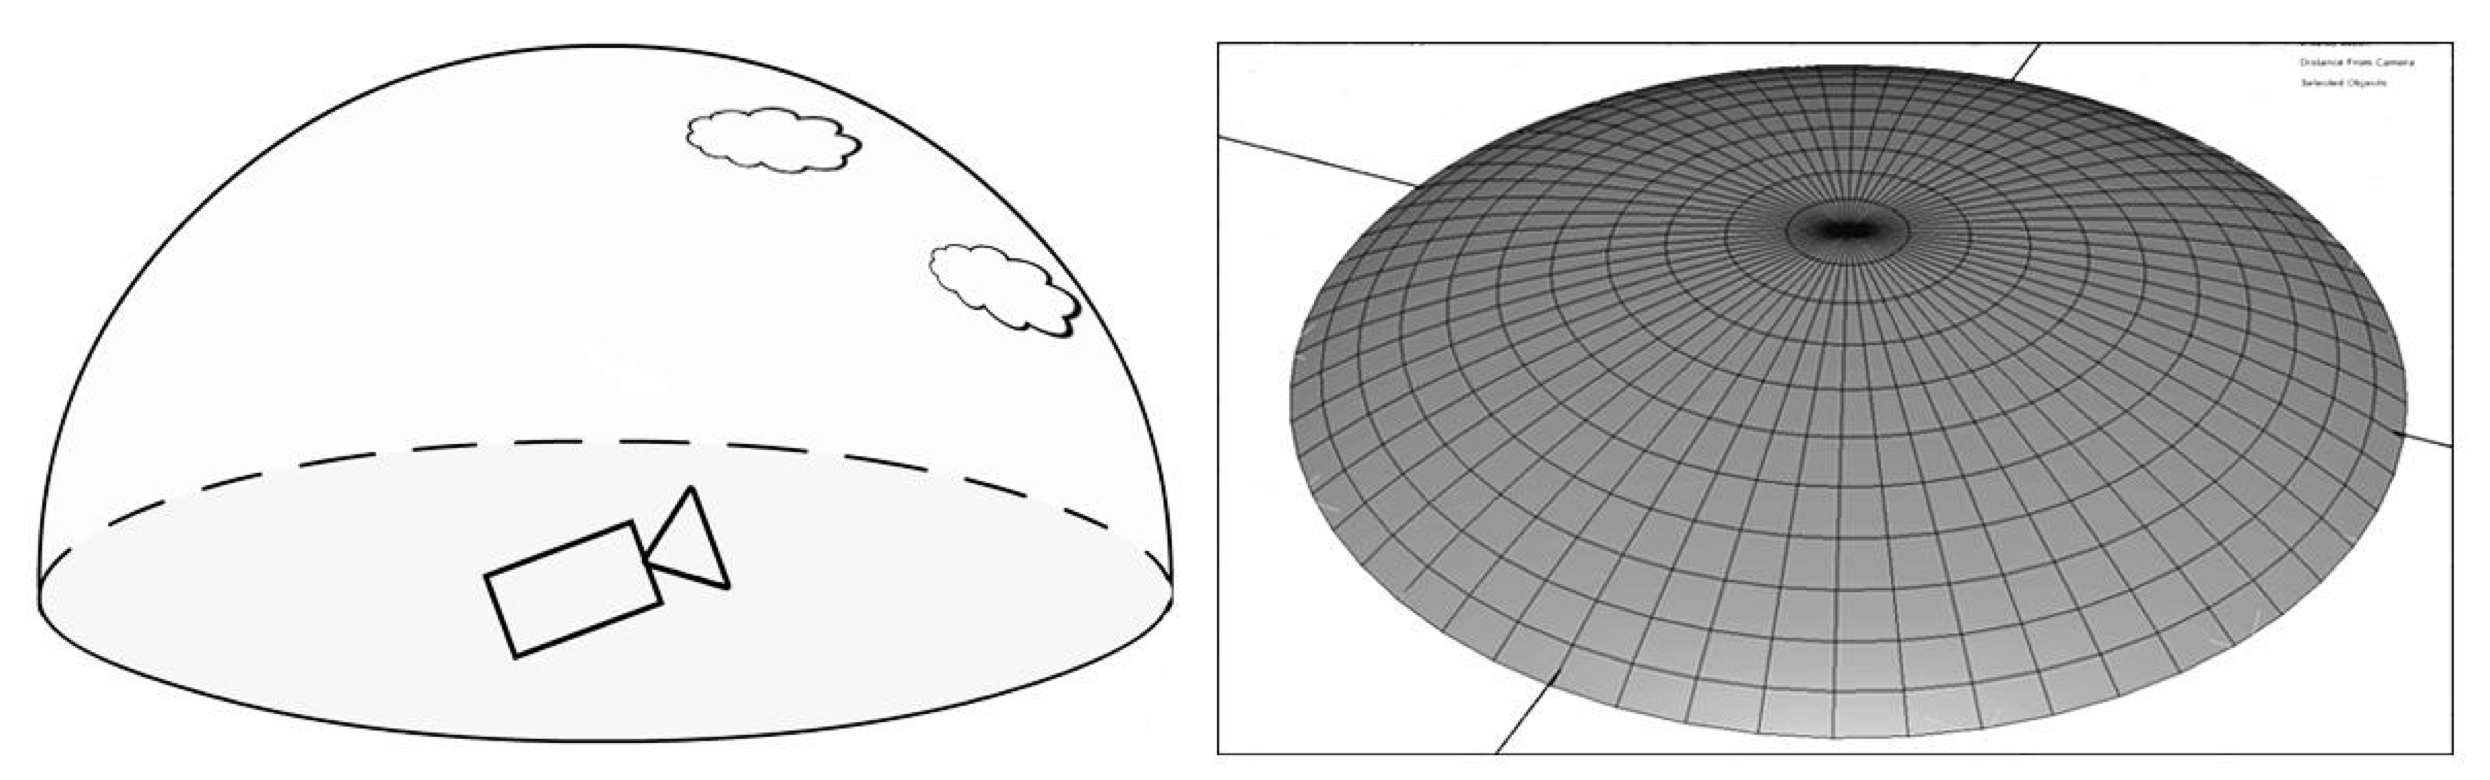
\includegraphics[scale=0.35]{img/skydome.png}
    \caption{Небосвод}
    \label{img:skydome}
\end{figure}

Participating media - это термин, используемый для описания объемов, заполненных частицами. Такими частицами могут быть крупные примеси,
такие как пыль, загрязнение, капли воды или просто молекулы.
В зависимости от своей плотности, media по-разному взаимодействуют со светом, который проходит между частиц и отскакивает от них.

\section{Обзор и анализ существующих программных систем и обоснование необходимости разработки}

\chapter{Конструкторский раздел}
\label{cha:design}

Необходимо на данных алгоритмах разработать генератор и визуализатор облаков.

\section{Функциональная модель}

На рисунках \ref{img:idef0} и \ref{img:idef0_1} видно функциональные модели для генерации и визуализации облака.

\begin{figure}[H]
    \centering
    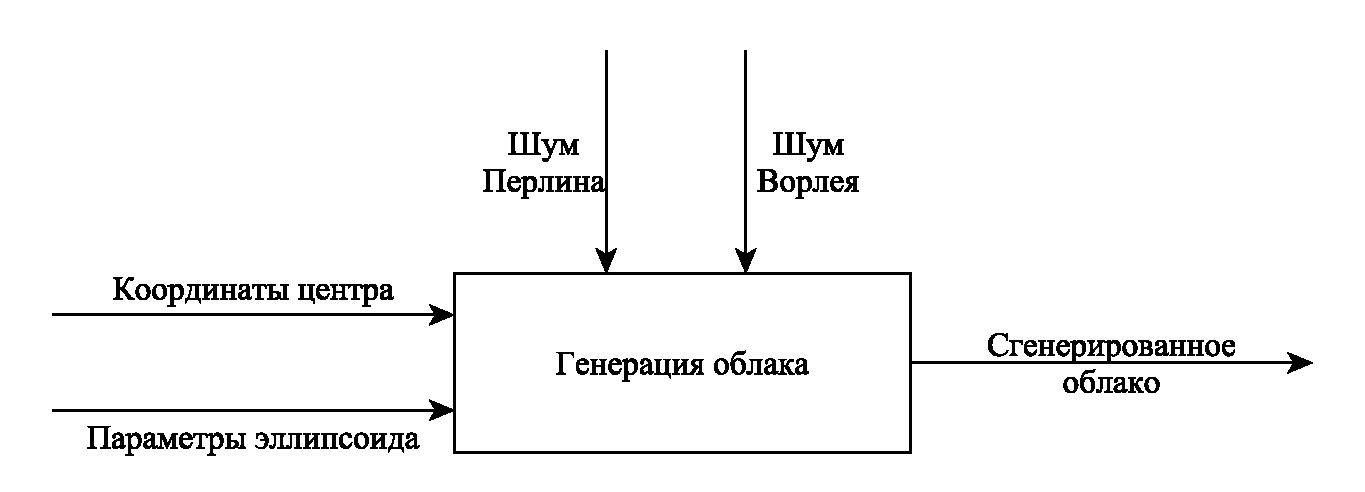
\includegraphics[scale=0.6]{img/idef0.pdf}
    \caption{Функциональная модель IDEF0 1 уровня для генерации облака}
    \label{img:idef0}
\end{figure}

\begin{figure}[H]
    \centering
    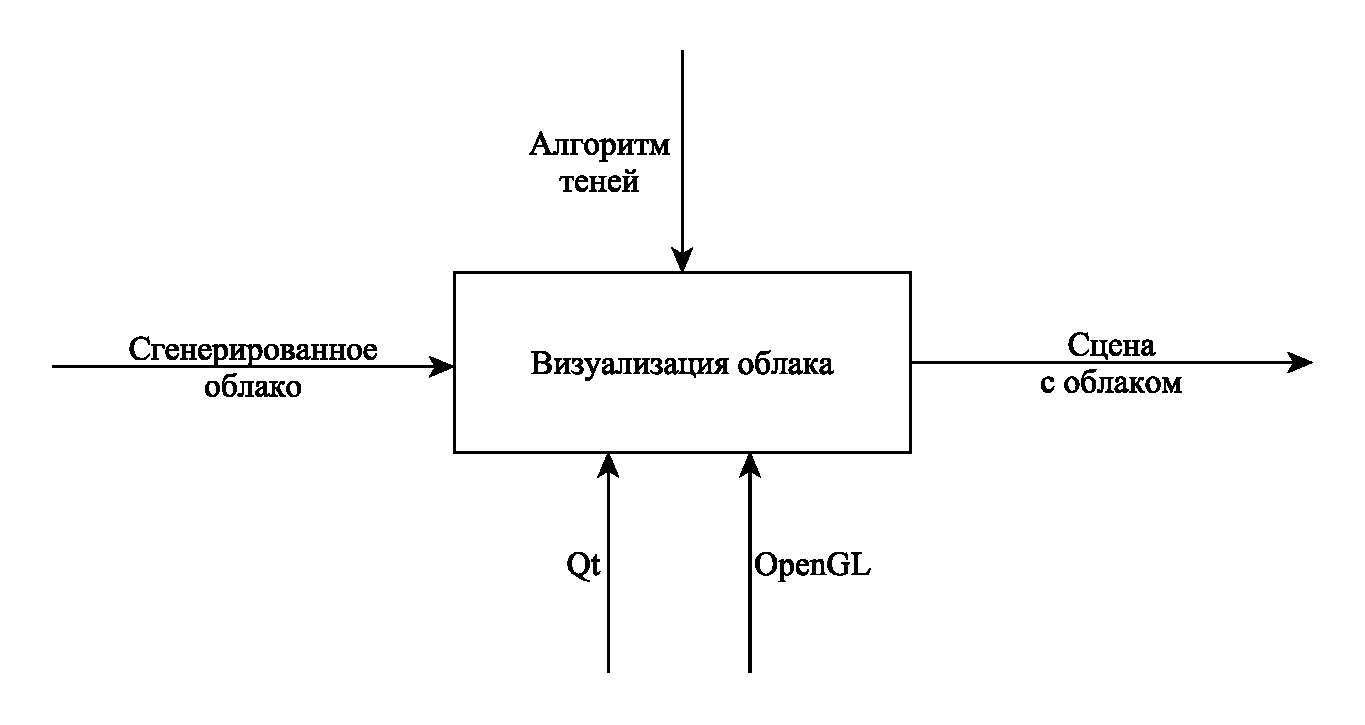
\includegraphics[scale=0.6]{img/idef0_1.pdf}
    \caption{Функциональная модель IDEF0 1 уровня для визуализации облака}
    \label{img:idef0_1}
\end{figure}

\section{Окружение}

Для создания окружающего пространства чаще всего используется куб больших размеров с наложенными текстурами.
Данный прием называется небесный куб. Куб создает впечатление об очень большом пространсве вокруг сцены и
существовании объектов, находящихся очень далеко \cite{SkyBox}.

\subsection{Форма облака}

Если из максимального значения интенсивности вычесть значение шума Уорли, можно получить результат как на рисунке \ref{img:worley2}

\begin{figure}[H]
    \centering
    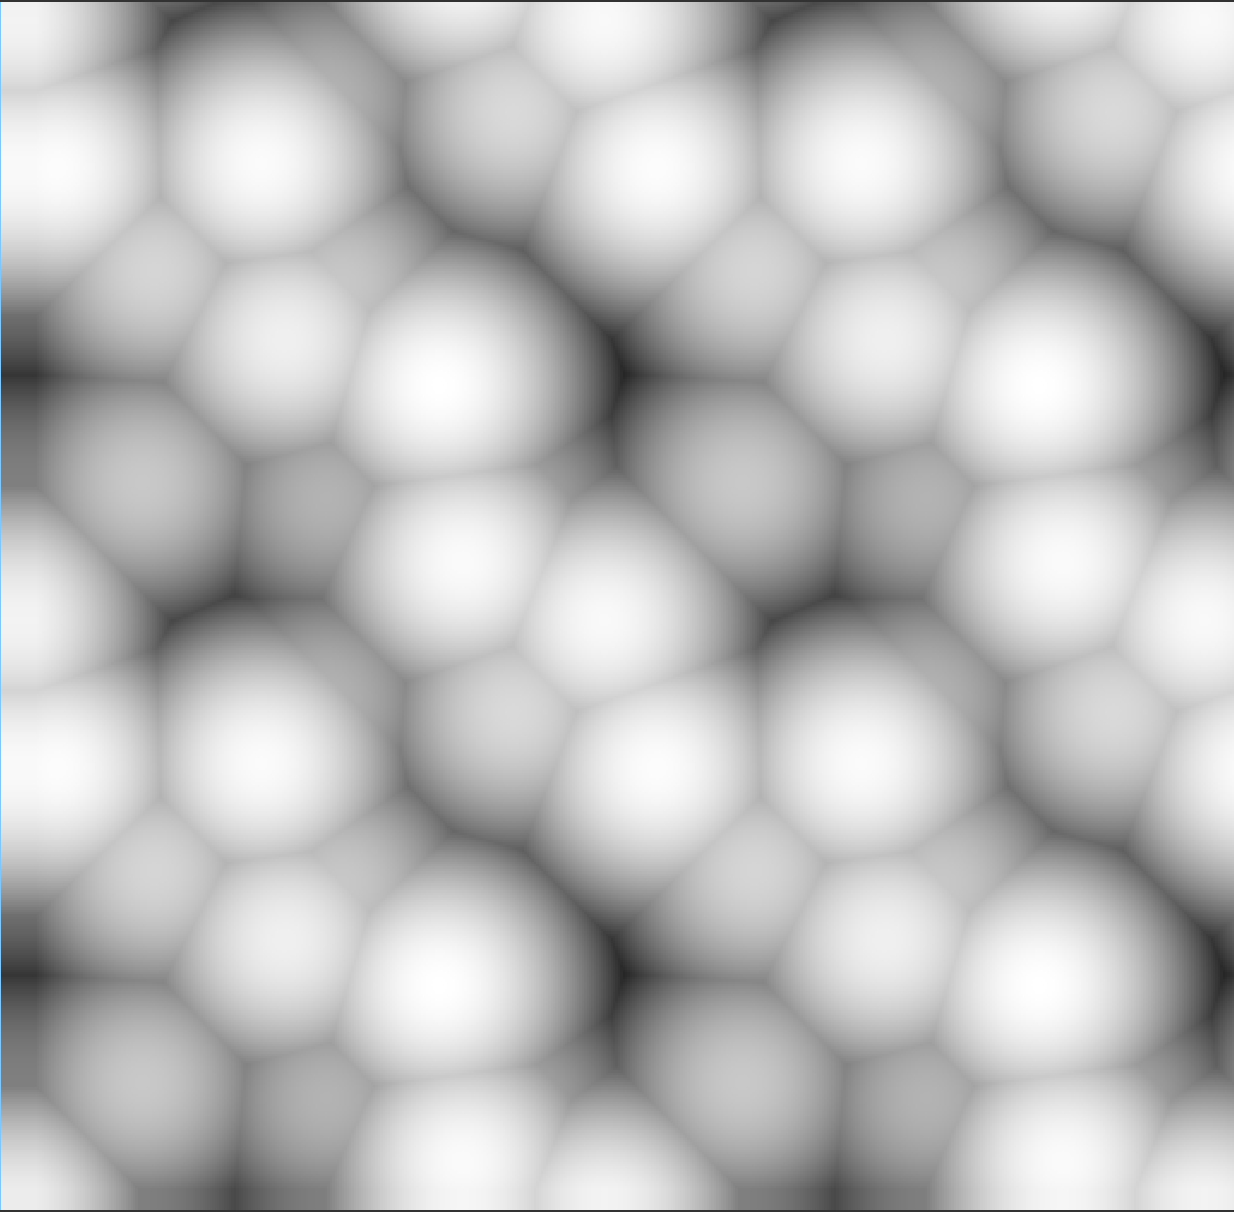
\includegraphics[scale=0.4]{img/worley2.png}
    \caption{Обратный шум Ворлея}
    \label{img:worley2}
\end{figure}

Если увеличить количество ячеек при генерации шума Уорли, можно получить результат как на рисунке \ref{img:worley3}.

\begin{figure}[H]
    \centering
    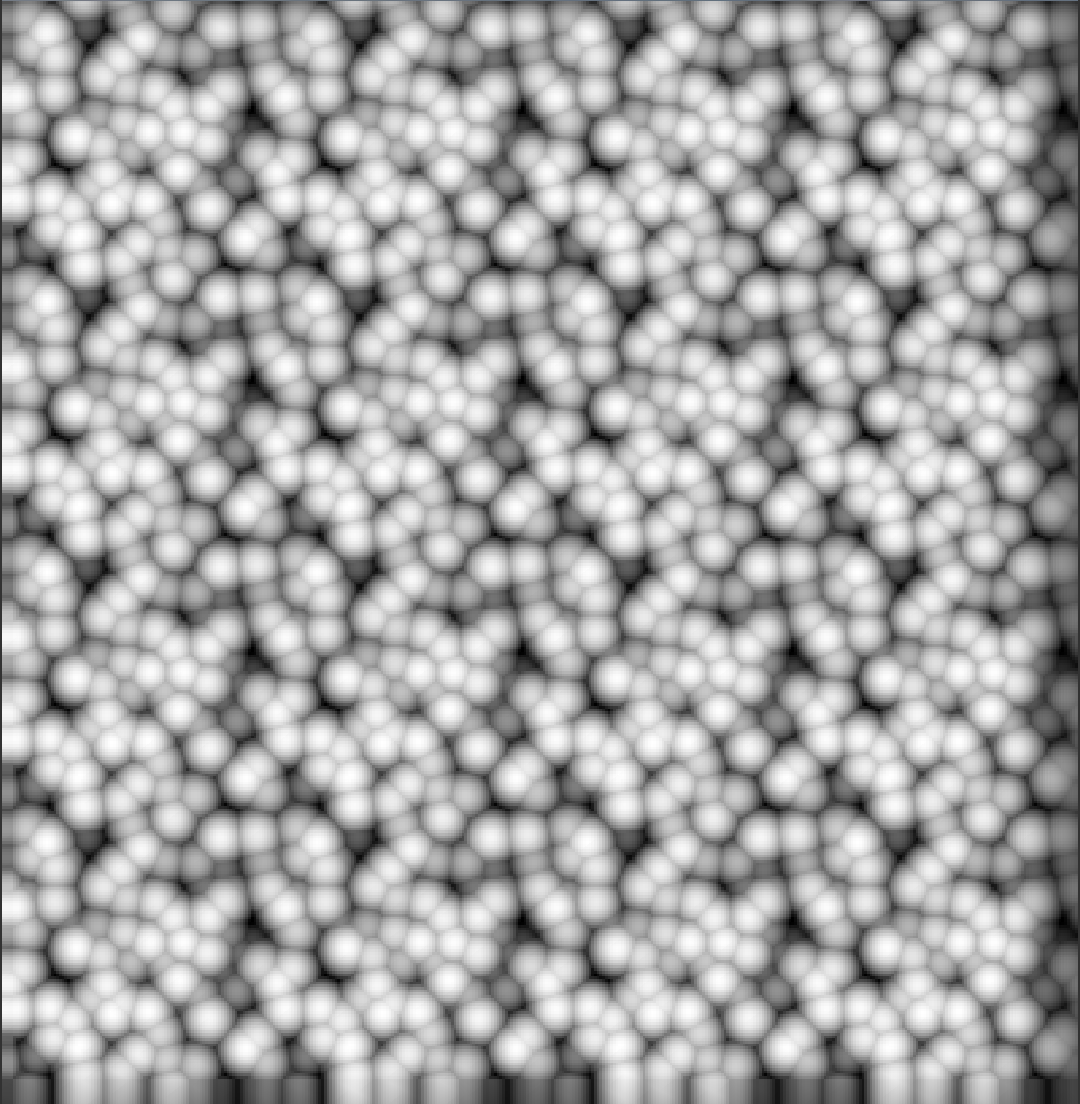
\includegraphics[scale=0.4]{img/worley3.png}
    \caption{Обратный шум Ворлея с большим количеством ячеек}
    \label{img:worley3}
\end{figure}

Для генерации облаков используется совмещение двух шумов. Шум Перлина придает
облаку случайную форму, а шум Ворлея - резкие очертания шарообразной формы.

Выведем формулу, в которой берется за основу шум Перлина, на который накладывается обратный шум Уорли первого варианта
(рисунок \ref{img:worley2}) и добавим к ним еще более мелкие шарики, взятые с шума Уорли, где больше ячеек (рисунок \ref{img:worley3}).
Экспериментальным методом была выведена данная формула \ref{eq:noise}.

\begin{equation}\label{eq:noise}
    \begin{matrix}
        F_{xyz} = P_{xyz}(20) + 0.1 + ((1 - W_{xyz}(4)) \cdot 1.5 - W_{xyz}(8) \cdot 0.7) \cdot 0.8 + P_{5x5y5z}(20), \\
        \text{где } P_{xyz}(n) - \text{ функция шума перлина после } n \text{ октав в точке } (x, y, z), \\
        W_{xyz}(n) - \text{ функция шума Уорли с плотностью ячеек } n \text{ в точке } (x, y, z) \\
    \end{matrix}
\end{equation}

Ее результат очень похож на облачную текстуру, которую можно увидеть на рисунке \ref{img:result_noise}.

\begin{figure}[H]
    \centering
    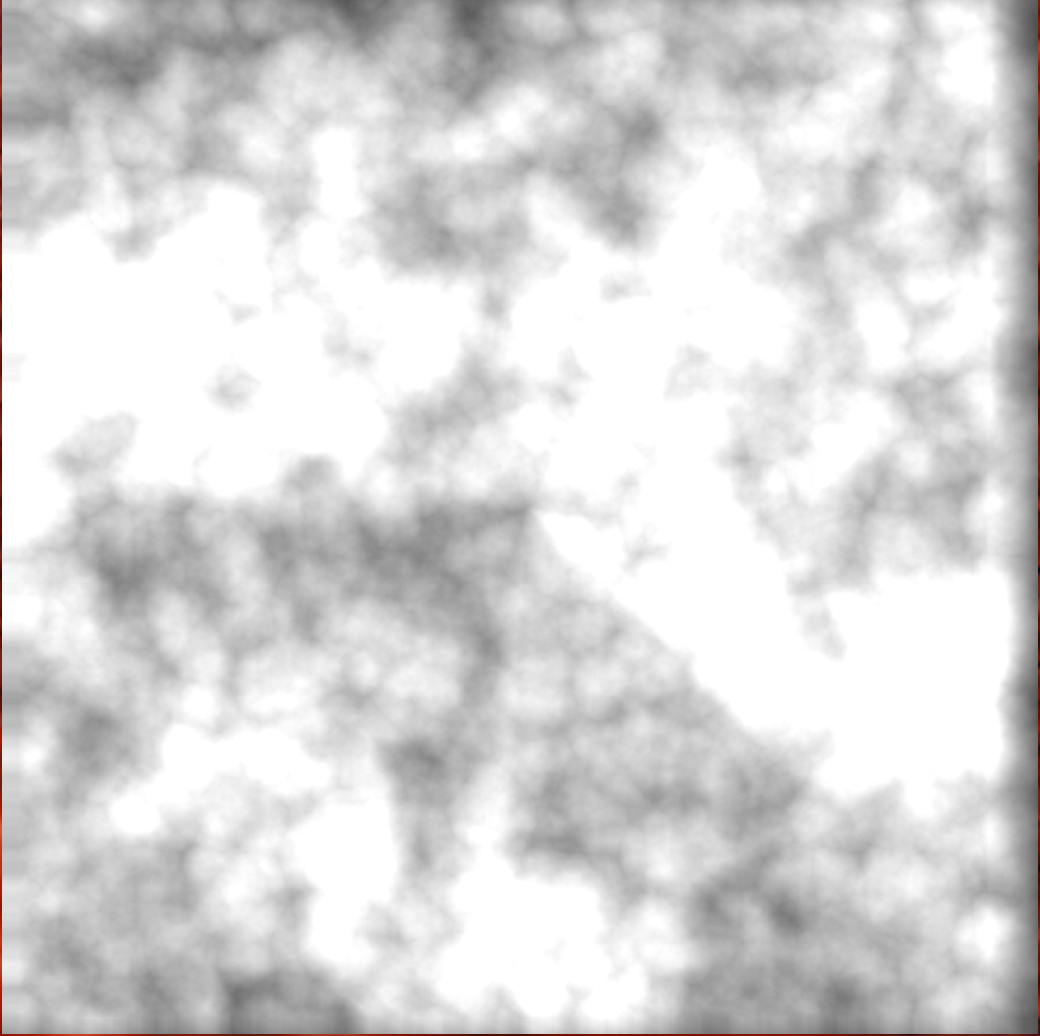
\includegraphics[scale=0.4]{img/result_noise.png}
    \caption{Результат объединения шумов}
    \label{img:result_noise}
\end{figure}

Для основы облака оспользуется параметрическое уранение эллипсоида, показанное на формуле \ref{eq:ellipsoid}
\cite{Ellipsoid}, в котором для каждой точки высчитывается новый радиус
по формуле \ref{eq:noise}. Поверхность эллипсоида получается очень похожей на облако.

\begin{equation}\label{eq:ellipsoid}
    \begin{cases}
        x = x_0 + a \cdot \sin(\Theta) \cdot \cos(\varphi) \\
        y = y_0 + b \cdot \sin(\Theta) \cdot \sin(\varphi) \\
        z = z_0 + c \cdot \cos(\Theta) \\
    \end{cases}
    , (-\frac{\pi}{2} \le \varphi \le \frac{\pi}{2}, 0 \le \Theta \le 2\pi)
\end{equation}

Параметры $a,b,c,x_0,y_0,z_0$ можно менять для получения разных размеров и местоположений облаков.

В зависимости от размеров облака, то есть от параметров $a, b, c$ выбирается шаг для углов $\Theta, \varphi$.
Поскольку размер каждой частицы составляет $0.1$, шаг был выбран $\frac{3}{\max(a,b,c)}$ для избежания
разрывов между частицами.

\section{Выводы}

Таким образом, был разработан алгоритм, основанный на шуме Перлина и шуме Уорли, которые влияют
на поверхность эллипсоида, получая объект, состоящий из частиц, который похож на облако.

\chapter{Технологический раздел}
\label{cha:impl}

Необходимо выбрать и обосновать выбранный язык программирования и средства разработки.
Разработать эффективно работающую струтуру программы и протестировать программу.

\section{Выбор и обоснование языка программирования}

Для визуализации большого количества частиц в реальном времени необходимо высокая производительность
используемых инструментов, а также удобный способ распараллеливания на видеокарту для повышения
скорости отрисовки. Был выбан язык программирования C++ с фреймворком Qt, в котором реализованы классы
для взаимодействия с OpenGL и шейерами \cite{QtOpenGL}.

\section{Интерфейс пользователя}

Интерфейс представлен на рисунке \ref{img:interface}

\begin{figure}[H]
    \centering
    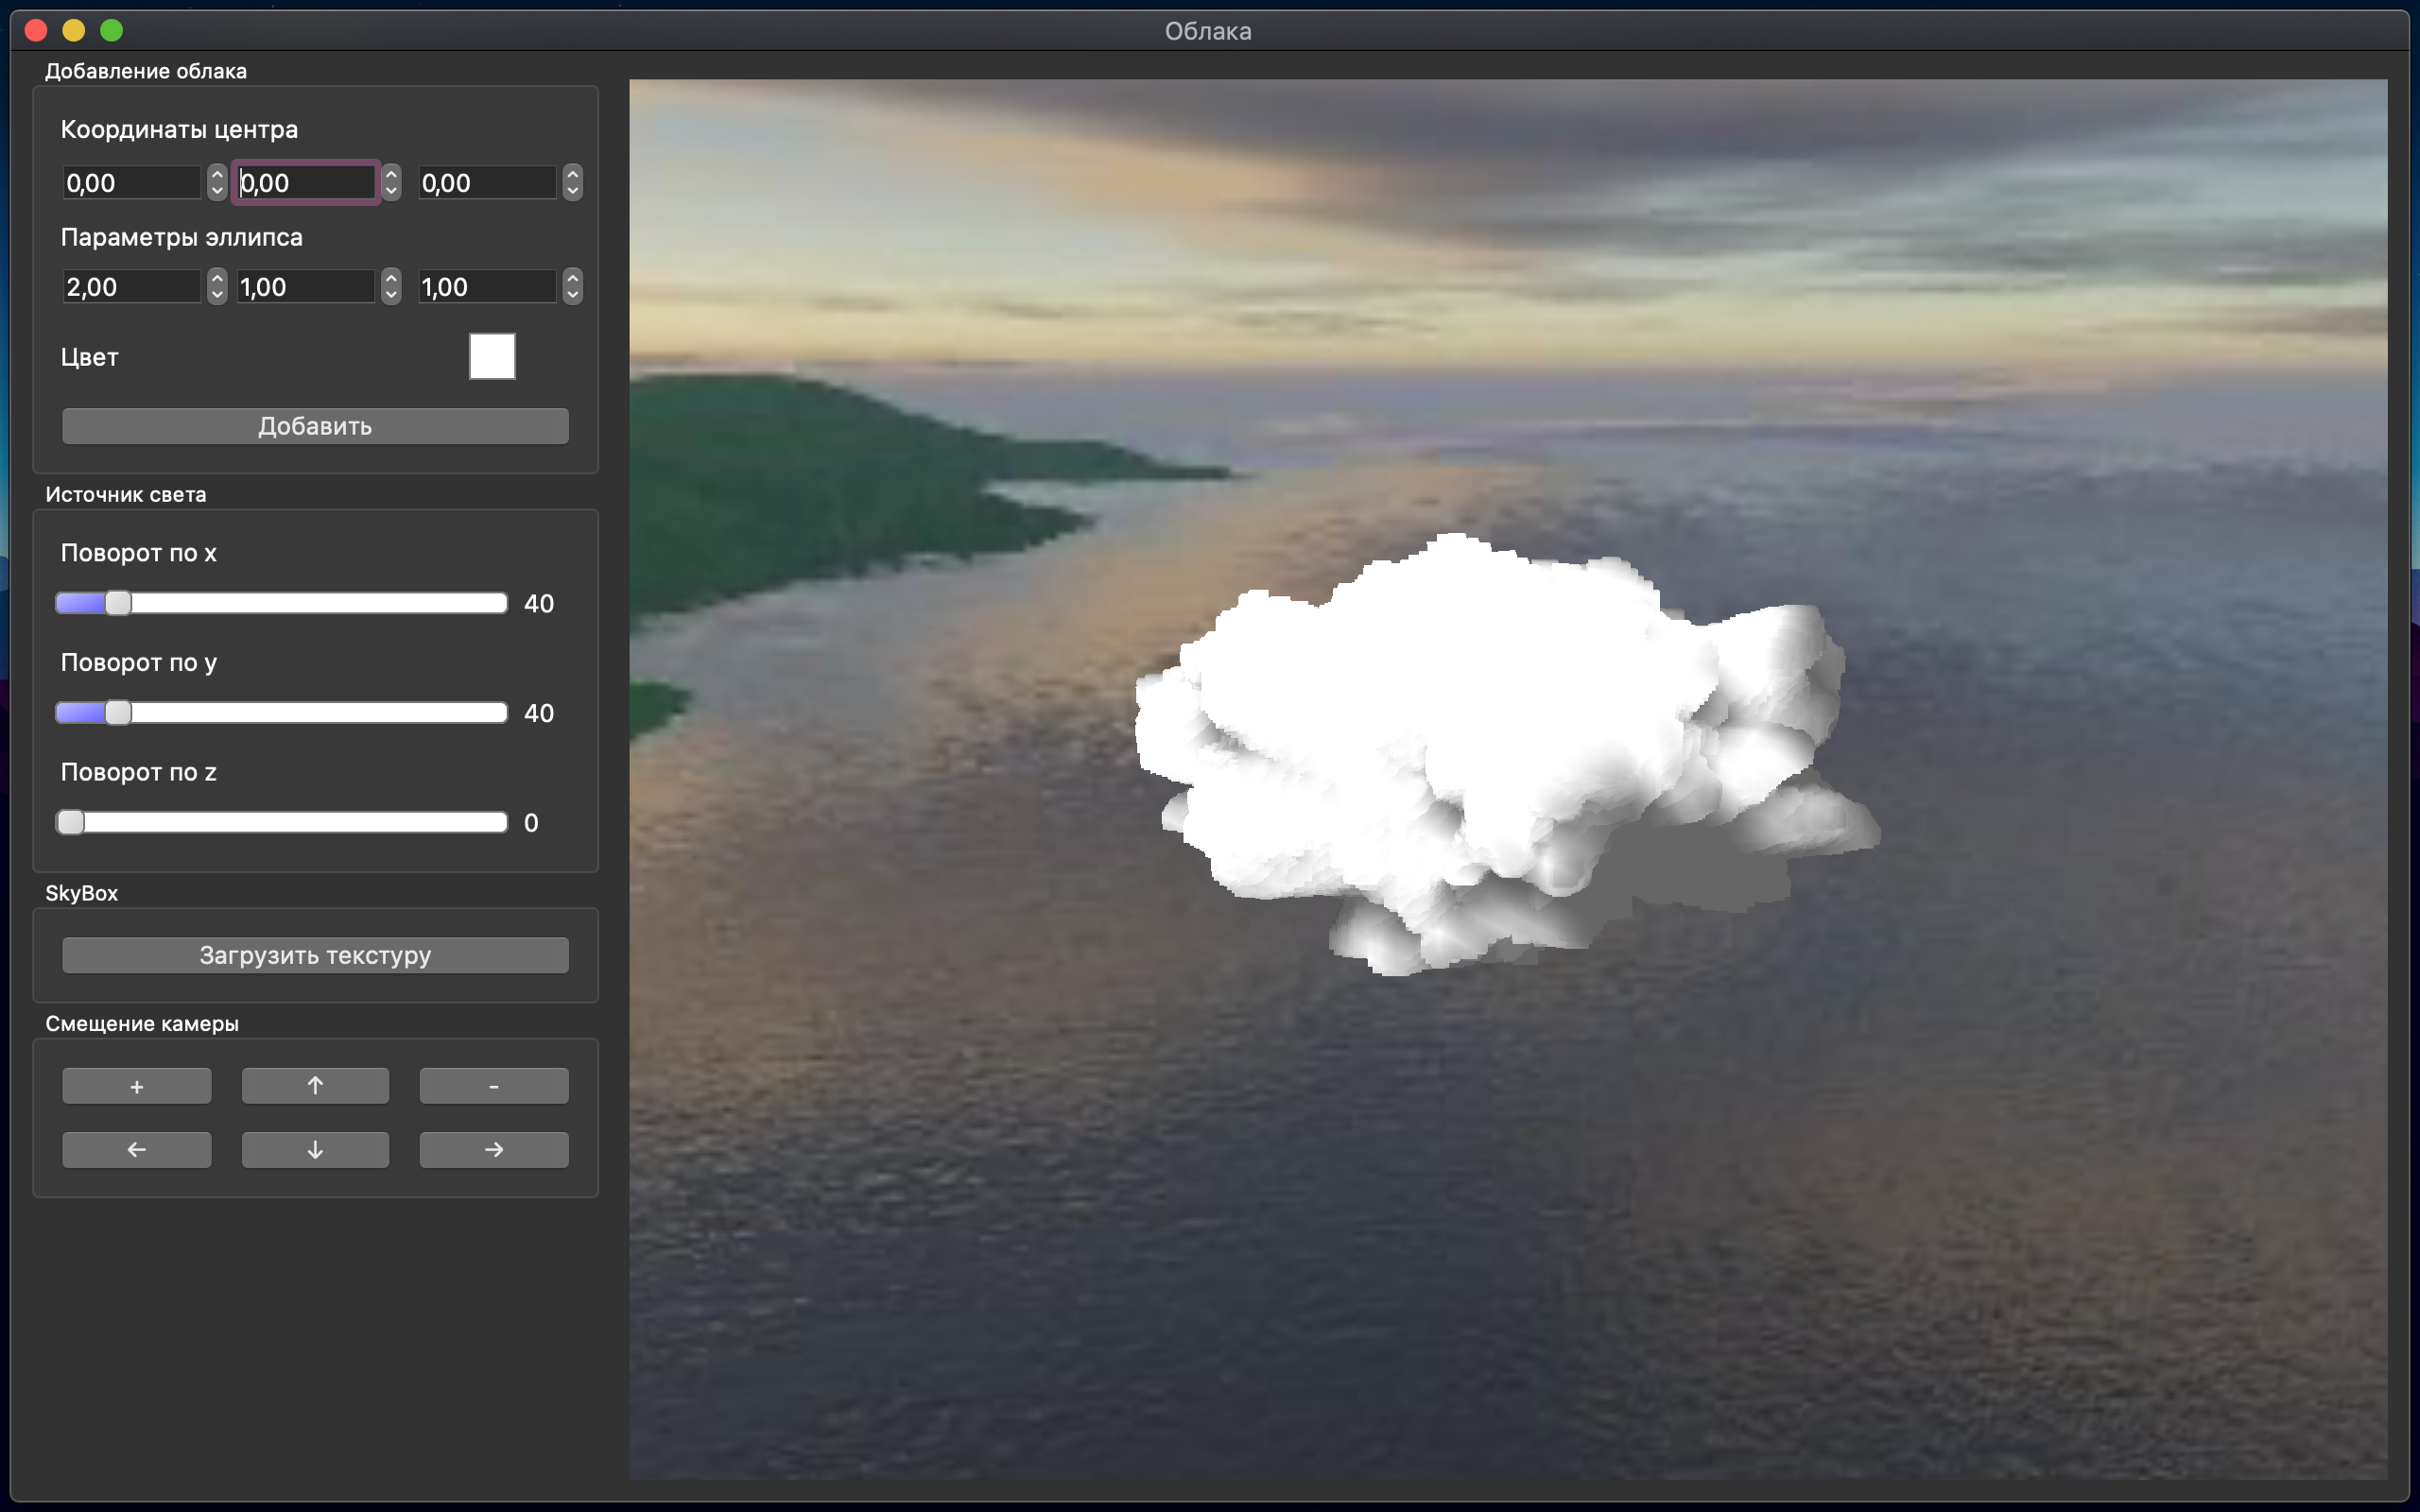
\includegraphics[scale=0.35]{img/interface.png}
    \caption{Интерфейс пользователя}
    \label{img:interface}
\end{figure}

Интерфейс позволяет добавлять облака с параметрами генерации, координатами центра и цветом.
Помимо этого имеется возможность вращать источник света вокруг центра системы координат с помощью ползунков.
Копки позволяют перемещать камеру по осям $x$ и $y$, а колесико мыши -- по $z$. Также с помощью мыши
можно вращать камеру вокруг центра координат.

\section{Хранение и обмен данными в системе}

Для хранения частиц используется класс частицы (таблица \ref{table:particle}).

\begin{table}[H]
    \centering
    \caption{Класс частицы}
    \label{table:particle}
    \begin{tabular}{|l|}
        \hline
        \multicolumn{1}{|c|}{\textbf{Particle}} \\
        \hline
        --\underline{arrayBuffer} : QOpenGLBuffer \\
        --\underline{indexBuffer} : QOpenGLBuffer \\
        --modelViewMatrix : QMatrix4x4 \\
        --r : float \\
        --g : float \\
        --b : float \\
        \hline
        +Particle( ) \\
        +Particle( x : float, y : float, z : float ) \\
        +Particle( x : float, y : float, z : float, r : float, g : float, b : float ) \\
        +\underline{initialization}( ) \\
        +\underline{firstDraw}( program : QOpenGLShaderProgram ) \\
        +draw( program : QOpenGLShaderProgram, functions : QOpenGLFunctions ) \\
        +setColor( r : float, g : float, b : float ) \\
        \hline
    \end{tabular}
\end{table}

\section{ER-модель}

При разработке приложения использован объекто-ориентированный подход. Модель классов
видно на рисунке \ref{img:er}

\begin{figure}[H]
    \centering
    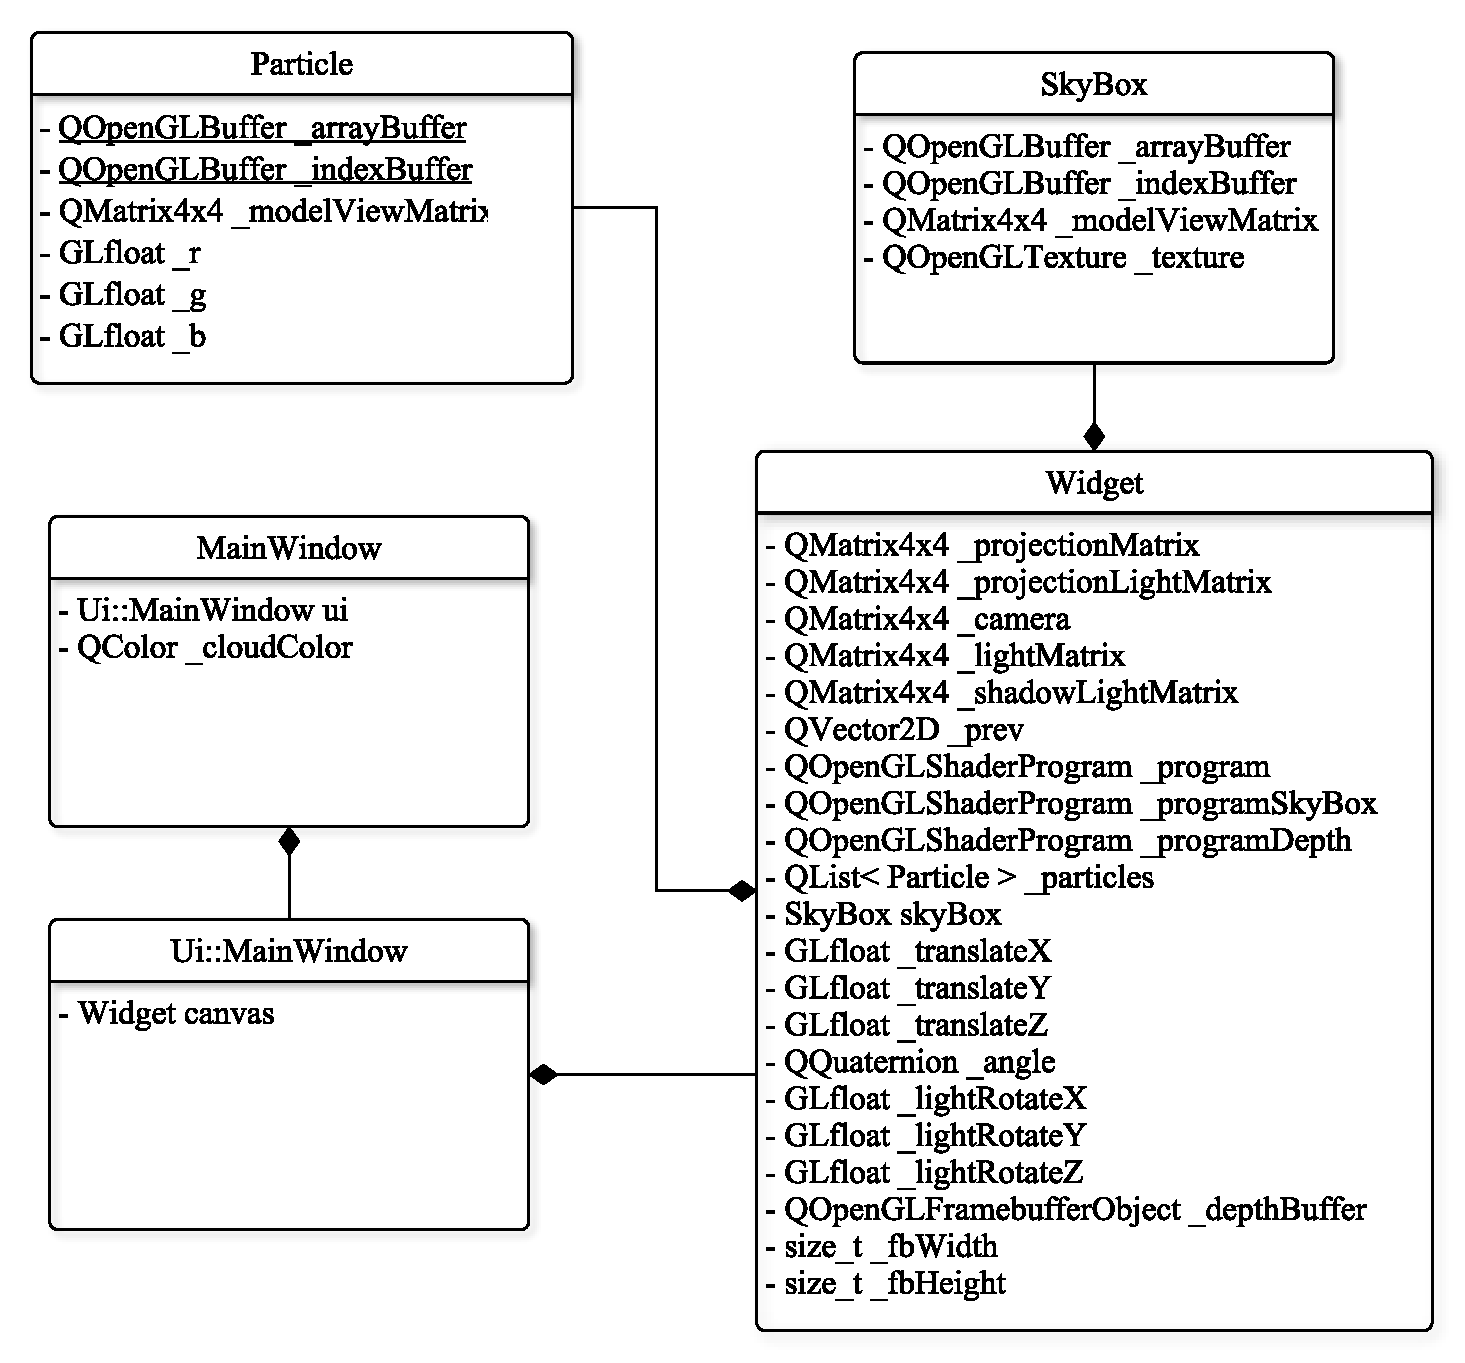
\includegraphics[scale=0.6]{img/er.pdf}
    \caption{ER-модель классов}
    \label{img:er}
\end{figure}

\section{Требования к аппаратуре}

Если необходимо визуализировать много облаков, требуется дискретная
видеокарта для комфортной частоты кадров.

\section{Тестирование}

Было проведено функциональное тестирование белого ящика, в ходе которого программа отработала
правильно. Также проведено тестирование пользовательского интерфейса, все элементы
интерфейса реагируют корректно.

\section{Выводы}

Был реализован алгоритм на выбранном языке C++. Программа полностью прошла функциональное тестирование
и тестирование интерфейса.

%%%% mode: latex
%%%% TeX-master: "rpz"
%%%% End:

\chapter{Исследовательский раздел}
\label{cha:research}

Тестирование программы проводилось на 2.7 GHz 2‑ядерном процессоре Intel Core i5 с встроенной видеокартой
Intel Iris Graphics 6100 на 1536 МБ и на 3.59 GHz 8-ядерном процессоре AMD Ryzen 7 3700x с дискретной
видеокартой NVidia GeForce RTX 2060 на 6144 МБ. В обоих случаях использовалось разрешение 1920 на 1080
точек.

\section{Исследование характеристик программы}

На рисунке \ref{img:plot} видна зависимость кадров в секунду от количества частиц.
В данном тесте проводилась визуализация облаков, каждое из которых состояло из 14400 частиц.

\begin{figure}[H]
    \begin{tikzpicture}
        \begin{axis}[
            legend pos = north east,
            xlabel=Количество частиц,
            ylabel=Кадры в секунду,
            grid = major,
            width = 0.8\paperwidth,
            height = 0.38\paperheight,
            line width = 1
        ]

            \legend{
                Встроенная видеокарта,
                Дискретная видеокарта
            };

            \addplot[color=black, mark=square] coordinates {
                    (0, 60)
                    (14400, 20)
                    (28800, 12)
                    (43200, 7)
                    (57600, 6)
                    (72000, 5)
                    (86400, 4)
                    (100800, 3)
                    (115200, 3)
                    (129600, 3)
                    (144000, 2)
            };

        \addplot[color=gray, mark=*] coordinates {
                    (0, 60)
                    (14400, 60)
                    (28800, 47)
                    (43200, 32)
                    (57600, 24)
                    (72000, 19)
                    (86400, 16)
                    (100800, 13)
                    (115200, 11)
                    (129600, 10)
                    (144000, 9)
            };
        \end{axis}
    \end{tikzpicture}
    \caption{Количество кадров в секунду в зависимости от количества частиц}
    \label{img:plot}
\end{figure}

\section{Примеры использования программы}

Пример работы программы при добавленном облаке видно на рисунке \ref{img:example1}.

\begin{figure}[H]
    \centering
    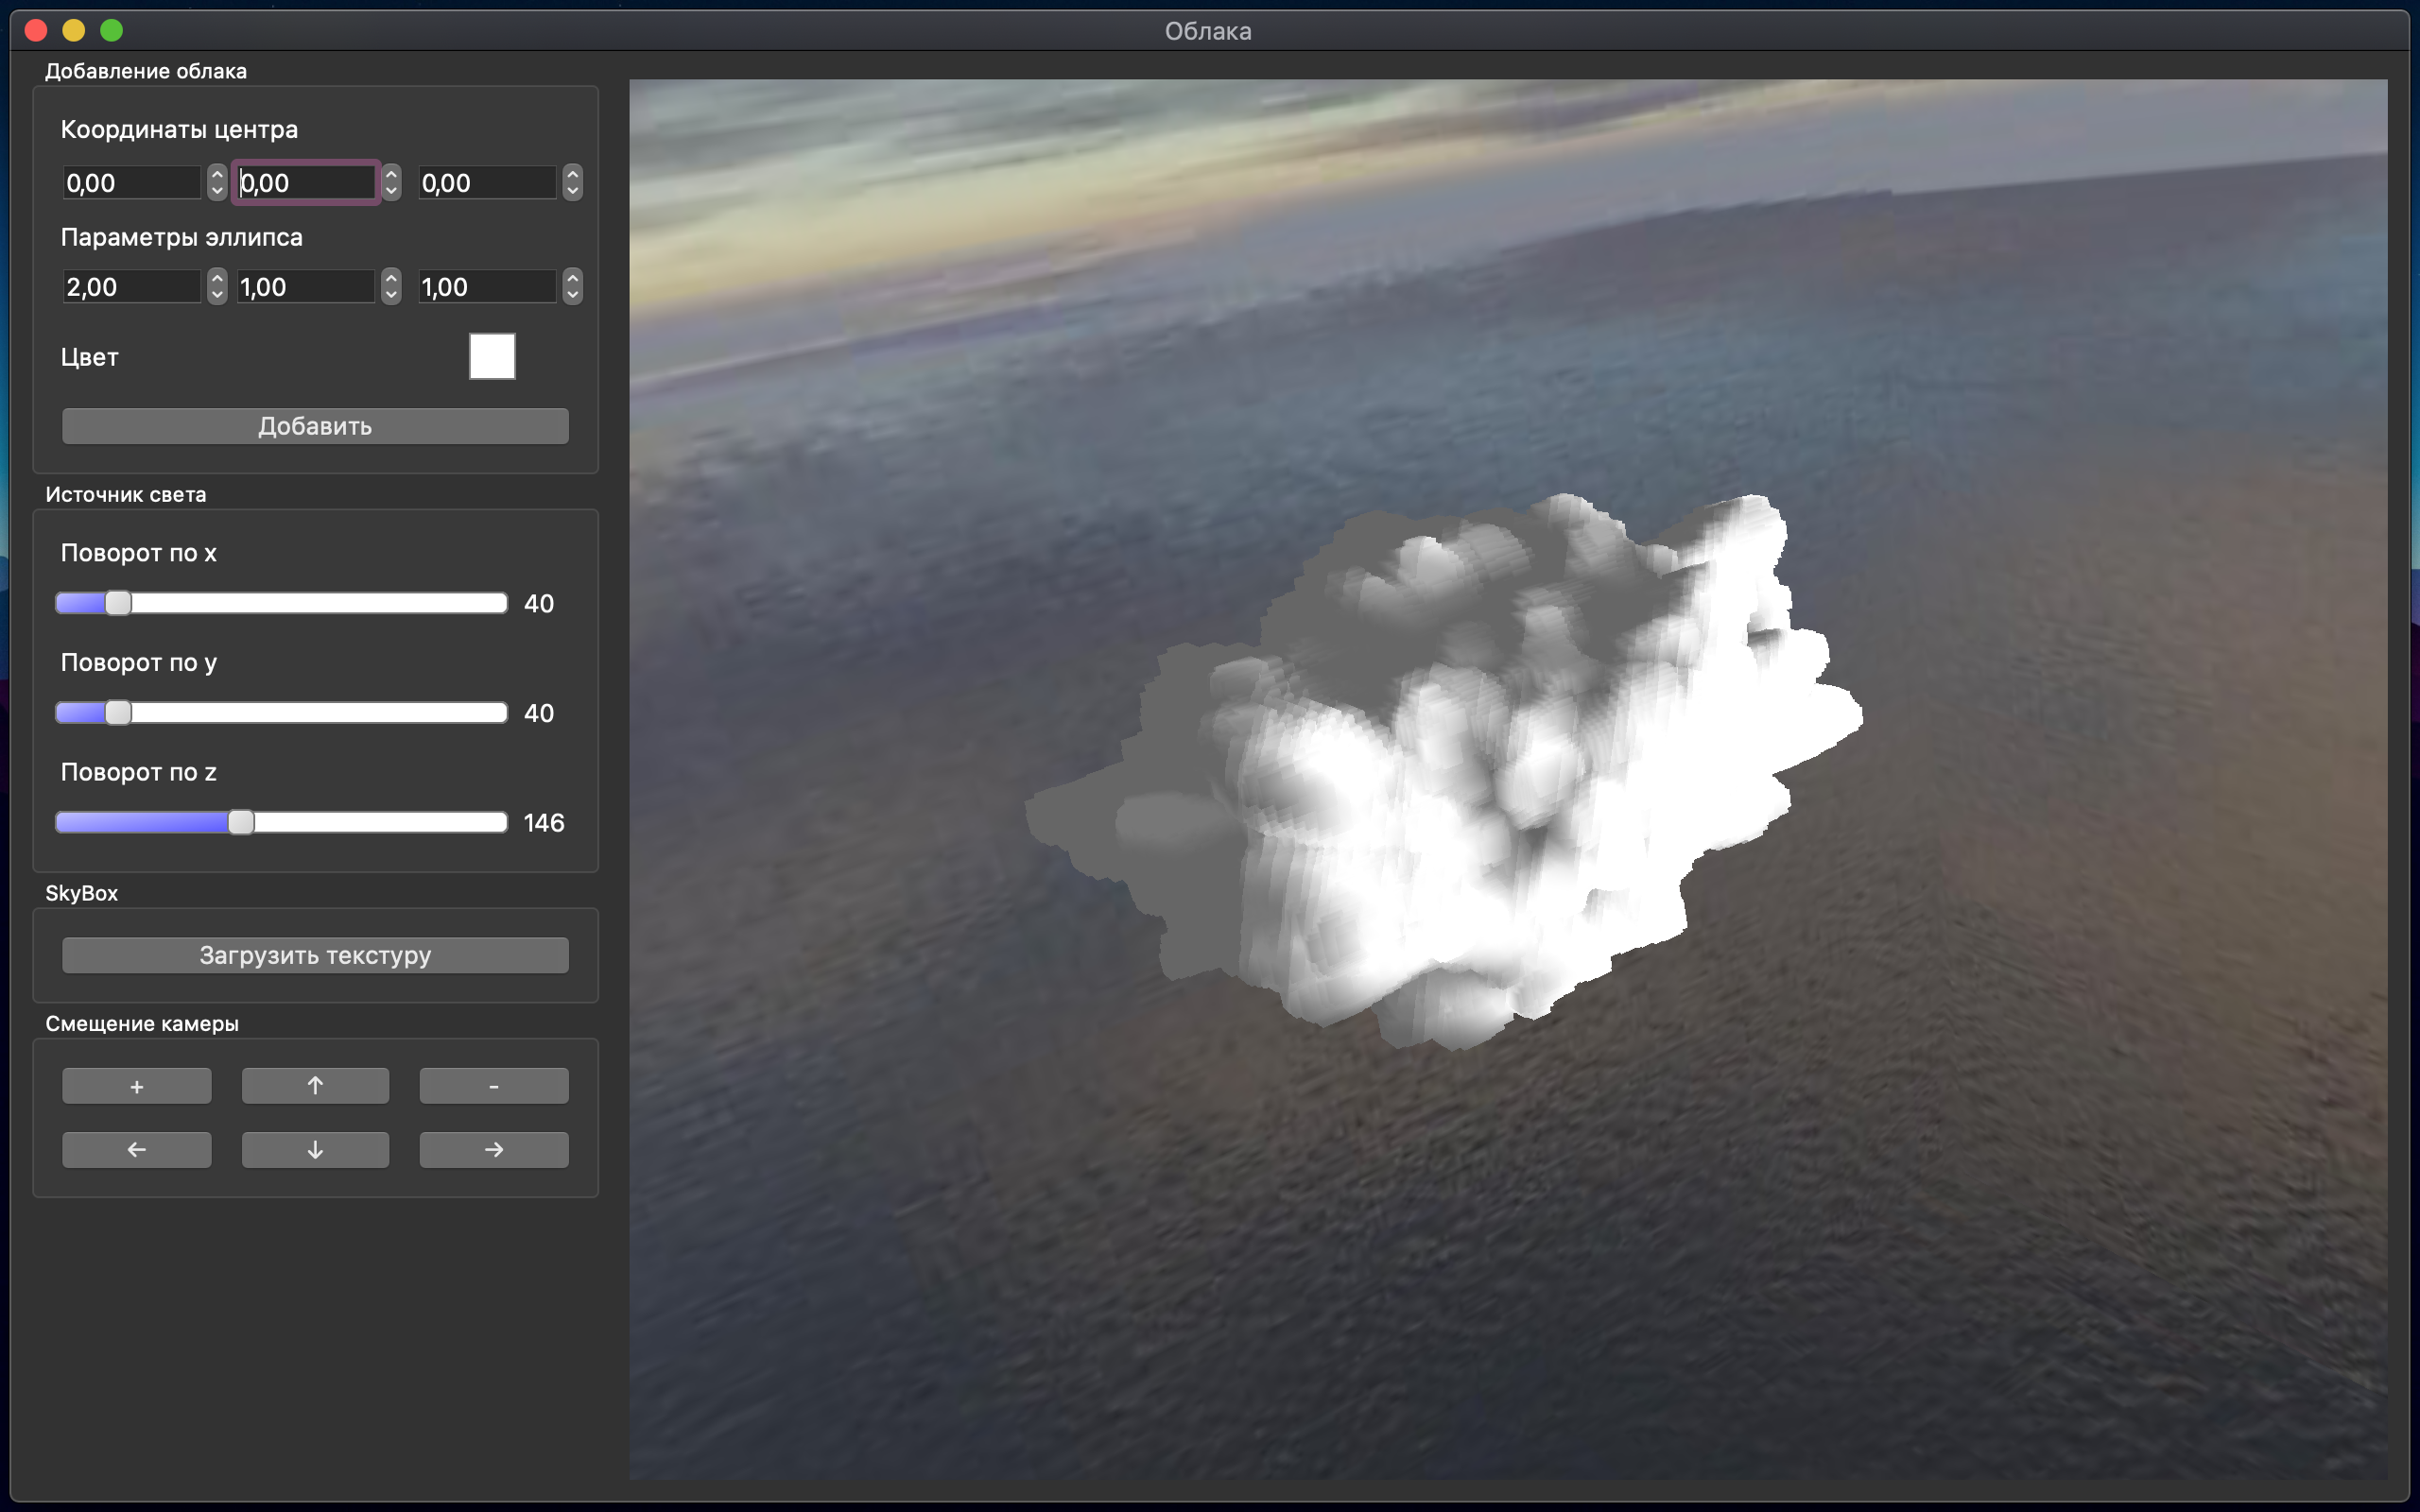
\includegraphics[scale=0.3]{img/example1.png}
    \caption{Пример добавленного облака}
    \label{img:example1}
\end{figure}

После добавления можно использовать камеру, чтобы рассмотреть облако с разных сторон и изменить положение
источника света (рисунок \ref{img:example2}).

\begin{figure}[H]
    \centering
    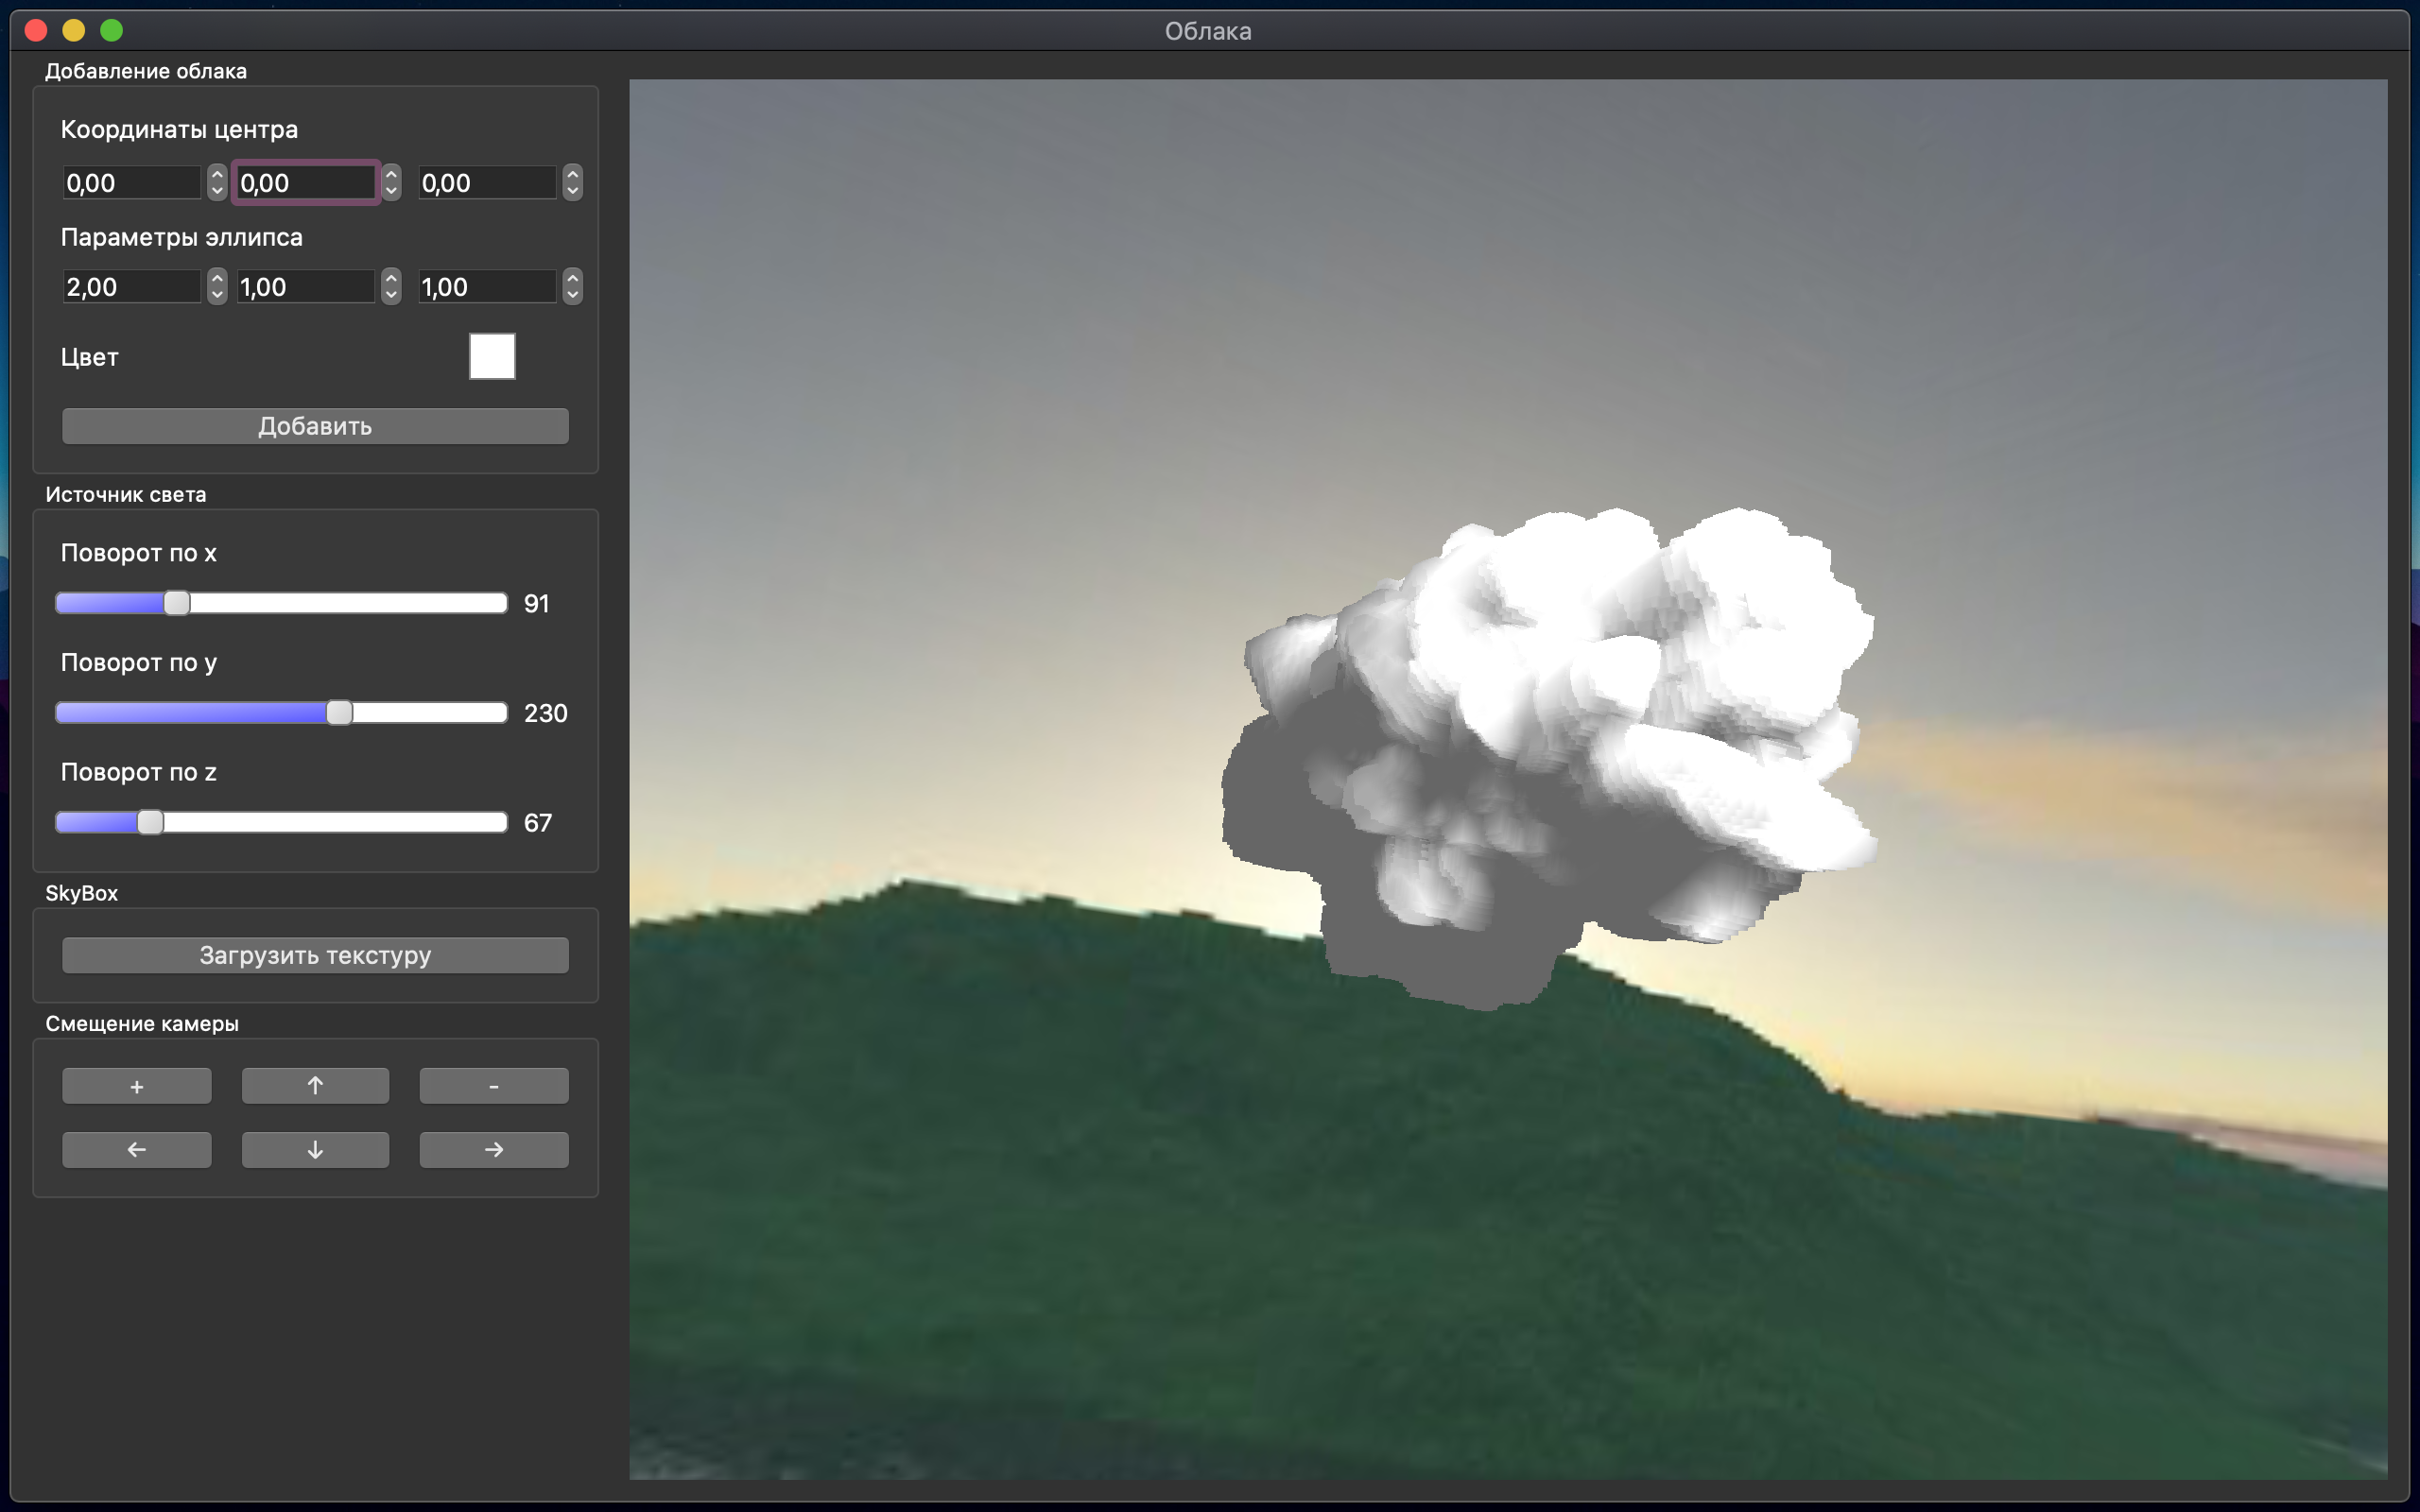
\includegraphics[scale=0.3]{img/example2.png}
    \caption{Пример работы камеры}
    \label{img:example2}
\end{figure}

Также можно поменять текстуру небесного куба, что видно на рисунке \ref{img:example3}.

\begin{figure}[H]
    \centering
    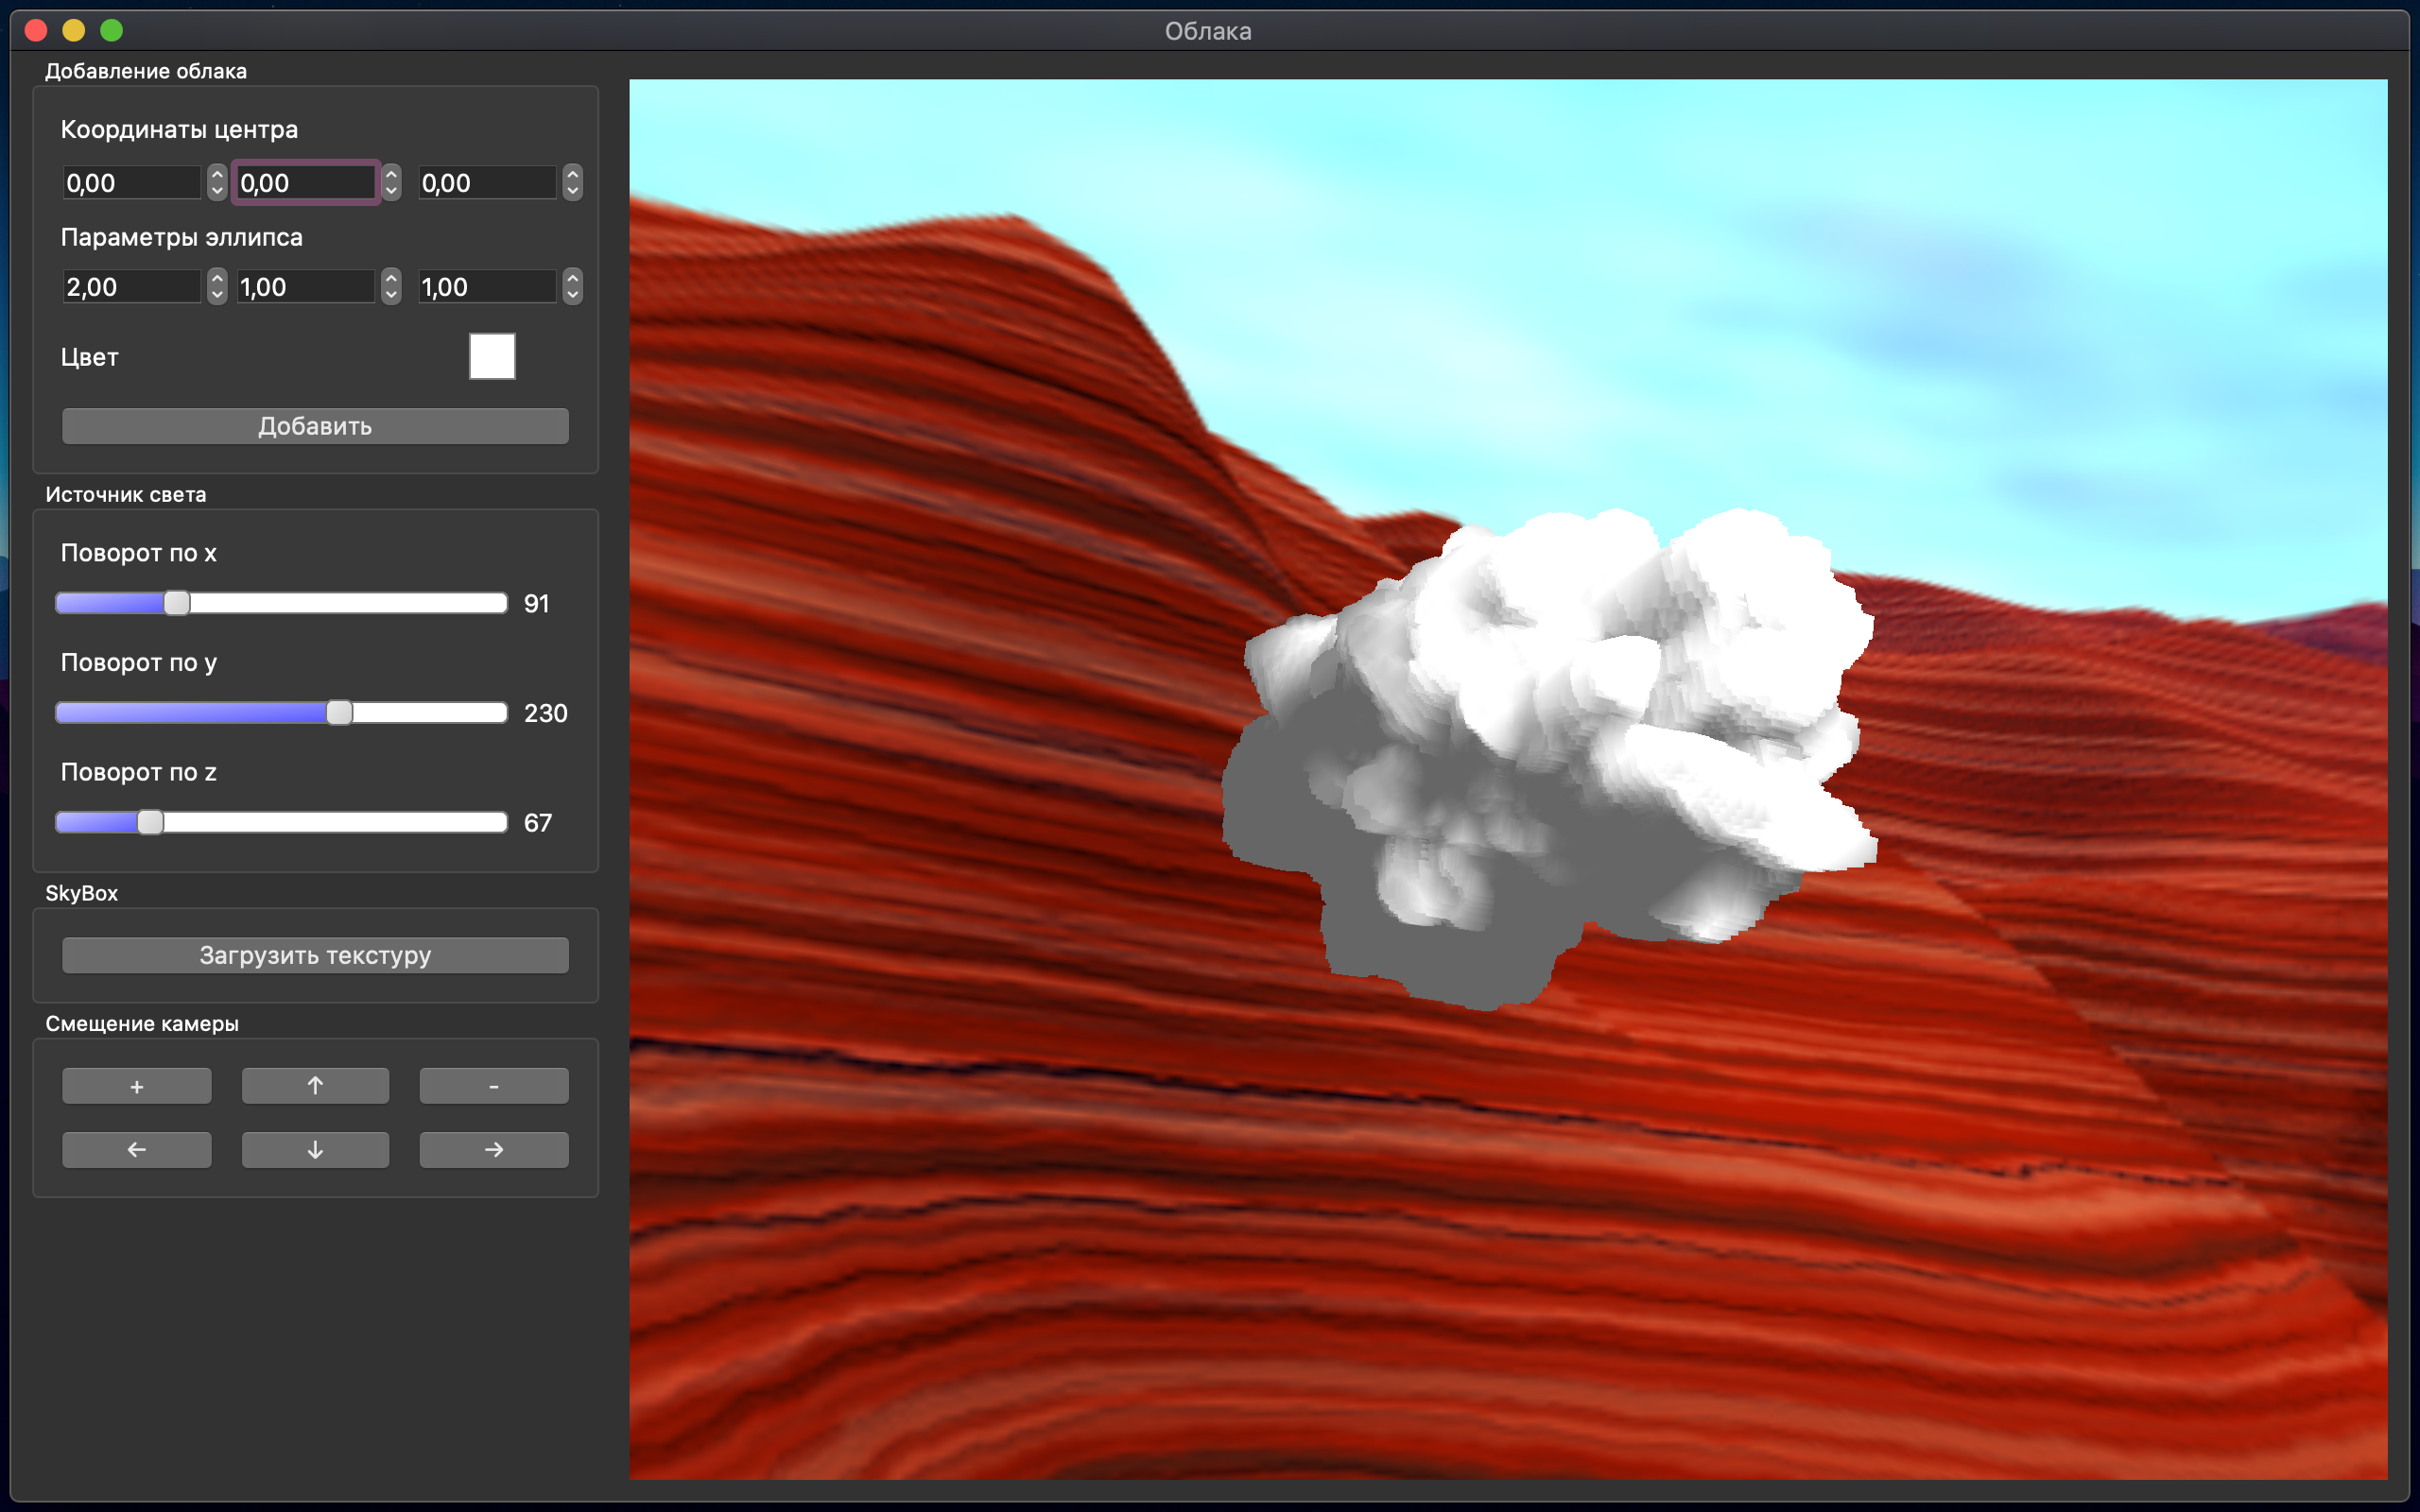
\includegraphics[scale=0.3]{img/example3.png}
    \caption{Пример смены небесного куба}
    \label{img:example3}
\end{figure}

\section{Выводы}

Если используется мощная дискретная видеокарта, то можно использовать до 50000 частиц, получая
частоту кадров больше 30. На встроенной видеокарте получился результат до 10000 частиц.


\backmatter %% Здесь заканчивается нумерованная часть документа и начинаются ссылки и
            
\Conclusion % заключение к отчёту

%% заключение


% % Список литературы при помощи BibTeX
% Юзать так:
%
% pdflatex rpz
% bibtex rpz
% pdflatex rpz

\bibliographystyle{ugost2008}
\bibliography{rpz}

%%% Local Variables: 
%%% mode: latex
%%% TeX-master: "rpz"
%%% End: 


%
%\appendix   % Тут идут приложения
%
%\chapter{Реализация и тестирование}

%
%\chapter{Еще картинки}
\label{cha:appendix2}
\blindtext

\begin{figure}
\centering
\caption{Еще одна картинка, ничем не лучше предыдущей. Но надо же как-то заполнить место.}
\end{figure}

%%% Local Variables: 
%%% mode: latex
%%% TeX-master: "rpz"
%%% End: 


\end{document}

%%% Local Variables:
%%% mode: latex
%%% TeX-master: t
%%% End:
